\documentclass{tufte-handout}

\title{Ultimate frisbee: strategy and tactics: O1}
\author[James Reynolds]{James Reynolds}

%\date{28 March 2010} % without \date command, current date is supplied

%\geometry{showframe} % display margins for debugging page layout

\usepackage{graphicx} % allow embedded images
  \setkeys{Gin}{width=\linewidth,totalheight=\textheight,keepaspectratio}
  \graphicspath{{graphics/}} % set of paths to search for images
\usepackage{amsmath}  % extended mathematics
\usepackage{booktabs} % book-quality tables
\usepackage{units}    % non-stacked fractions and better unit spacing
\usepackage{multicol} % multiple column layout facilities
\usepackage{lipsum}   % filler text
\usepackage{fancyvrb} % extended verbatim environments
  \fvset{fontsize=\normalsize}% default font size for fancy-verbatim environments

% Standardize command font styles and environments
\newcommand{\doccmd}[1]{\texttt{\textbackslash#1}}% command name -- adds backslash automatically
\newcommand{\docopt}[1]{\ensuremath{\langle}\textrm{\textit{#1}}\ensuremath{\rangle}}% optional command argument
\newcommand{\docarg}[1]{\textrm{\textit{#1}}}% (required) command argument
\newcommand{\docenv}[1]{\textsf{#1}}% environment name
\newcommand{\docpkg}[1]{\texttt{#1}}% package name
\newcommand{\doccls}[1]{\texttt{#1}}% document class name
\newcommand{\docclsopt}[1]{\texttt{#1}}% document class option name
\newenvironment{docspec}{\begin{quote}\noindent}{\end{quote}}% command specification environment

\begin{document}

\maketitle% this prints the handout title, author, and date


\begin{marginfigure}%
  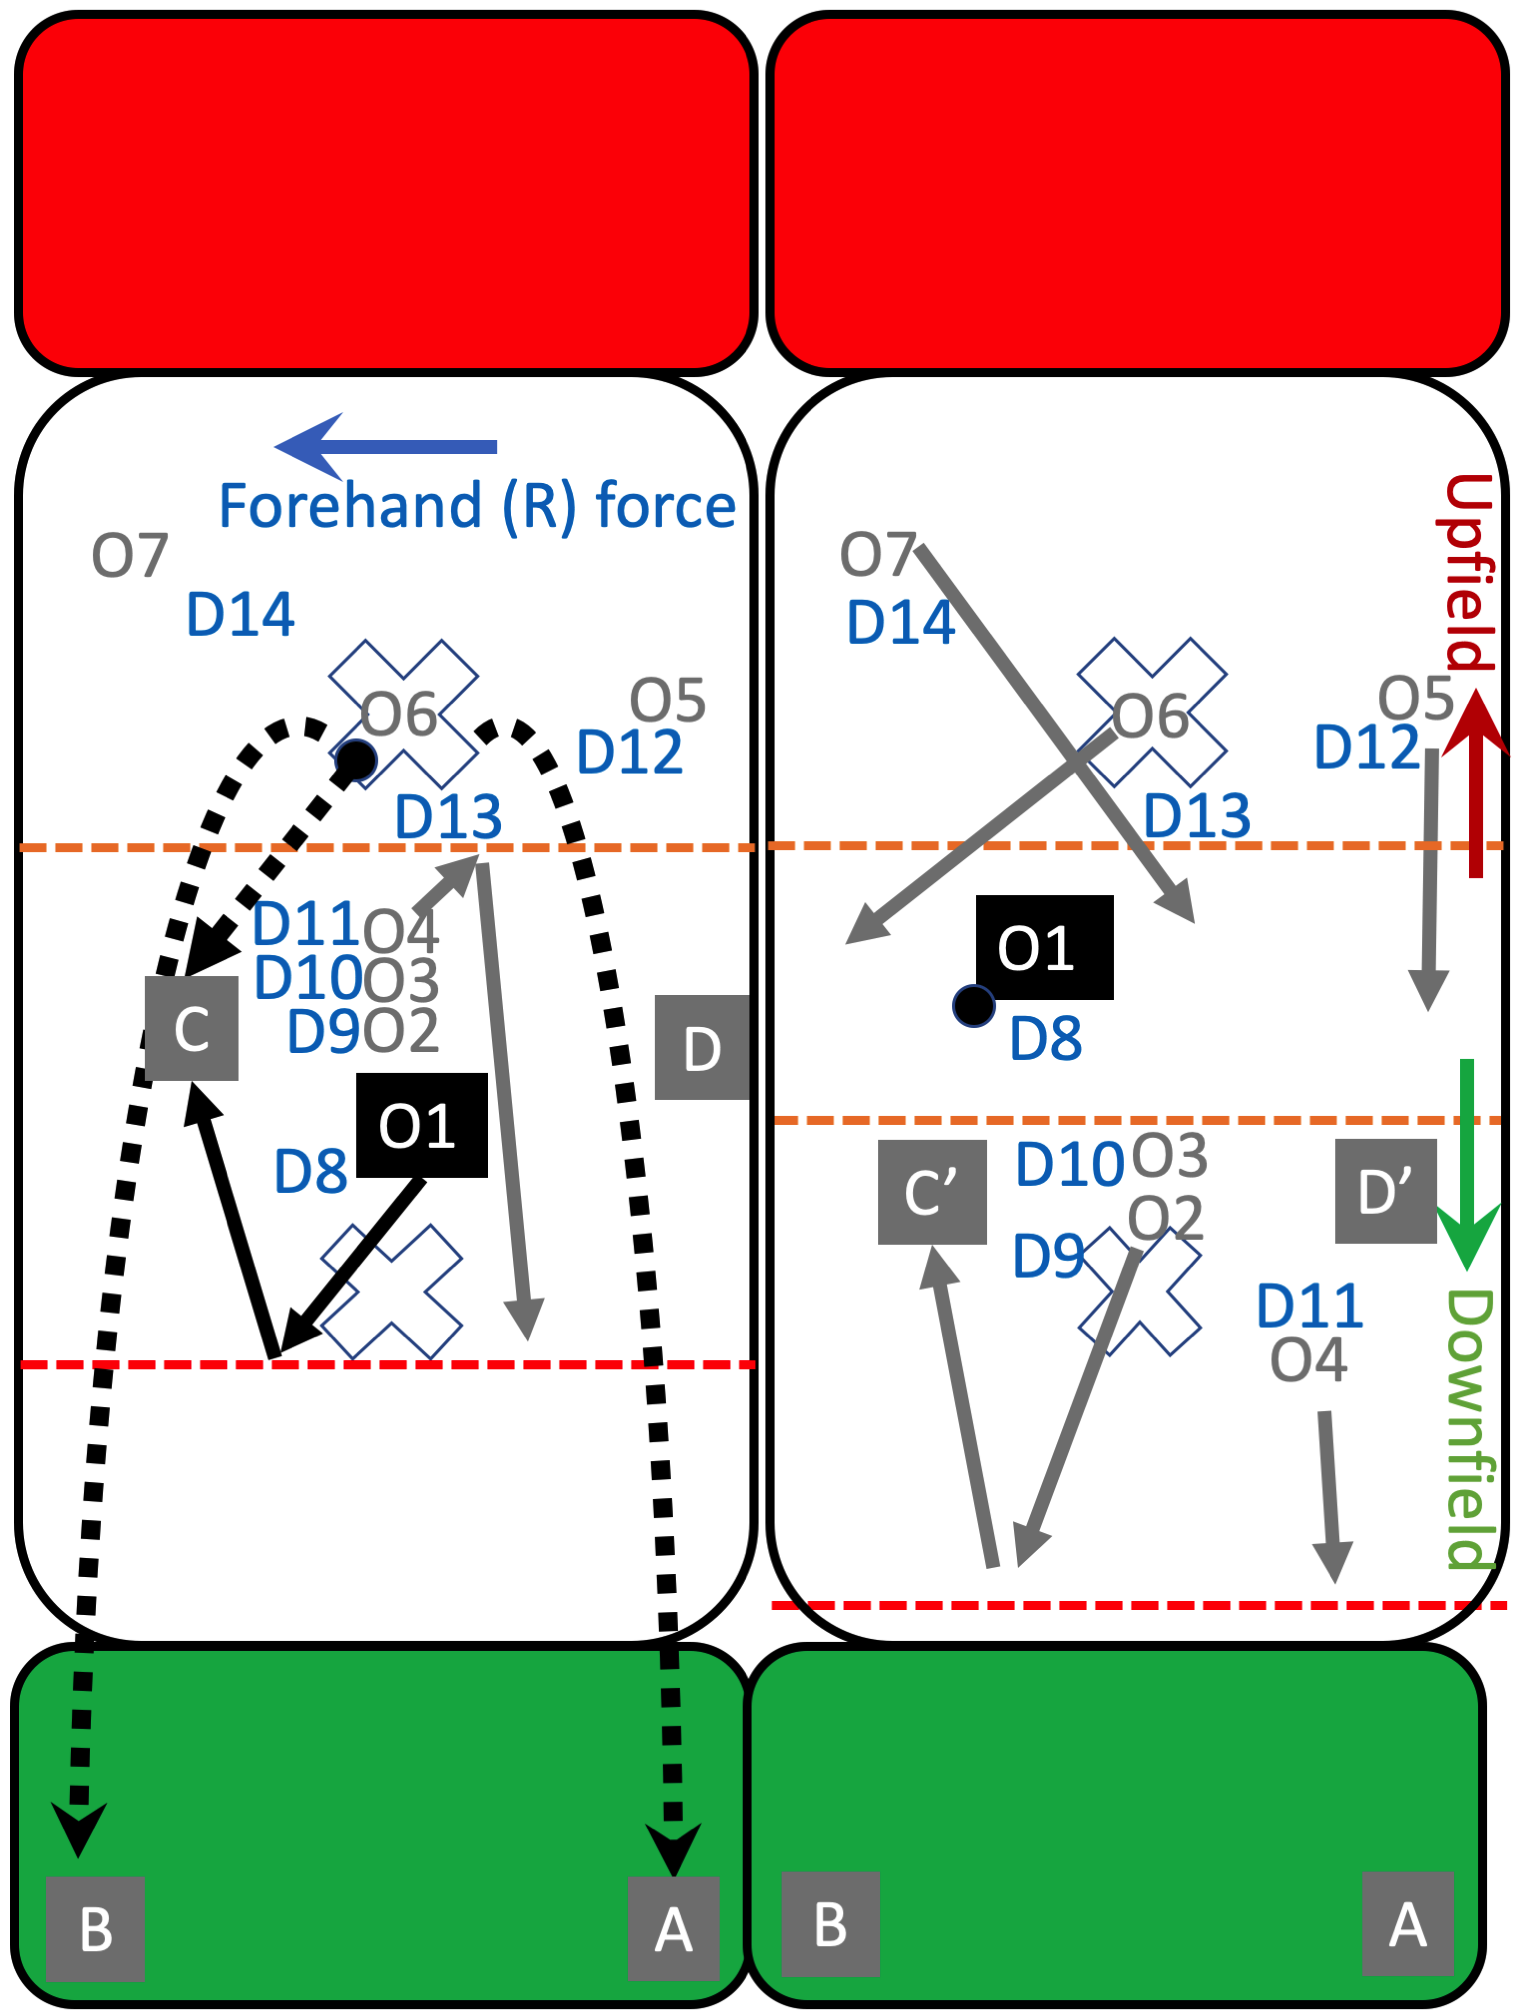
\includegraphics[width=\linewidth]{O1-vertical}
  \caption{Vertical stack formation}
  \label{fig:O1-vertical}
\end{marginfigure}



%\printclassoptions
This document is about 
playing primary 'middle' 
or left wing 
on offence. 
These are
referred to as position O1 here\footnote{This document
is part of a series, 
the rest of which is available here (LINK TO BE PROVIDED}.
\newthought{Your team is starting the point} on offence.
There are three key pieces of information you'll need from your team before the point starts:
1) What everyone's role is? 
(You are O1, 
which makes you a cutter\footnote{  
O2, O3 and O4 are also cutters, and
O5, O6 and O7 are handlers.}.;
2) What offensive structure/plan is your team planning on using?\footnote{
Vertical,
horizontal, 
or something else}
3) What defensive structure/plan to use if there is a turnover? 

What actually happens, 
however, 
is likely to depend more on 
what the opposing team (D1-D7) does. 
After the pull 
as you run downfield\footnote{
In the meantime, 
the handlers on your team 
will be busy 
catching the pull
Figures \ref{fig:O1-vertical} and  \ref{fig:O1-horizontal} 
show O6 starting play 
at the brick mark, 
as might occur if 
the pull is out.} it will help 
if you can figure out 
what defensive structure the D team use.
It might be:
person-match defence;
a zone defence; or
something else
(often called "junk").
What you should do 
in the event of each
is the subject of this document. 


\section{Person-match defence, vertical stack}\label{sec:vertical}
So, if you identify the defensive structure as person-match
the next thing to try and figure out
is what direction the opposition are forcing. 
\smallcaps{Forehand force} for right handers is the most common, 
so this is discussed first. 

Three throws for O6 
to get the disc 
to you are:
\begin{enumerate}
\item a break-side 
huck to A\footnote{
This throw is 
probably
very difficult for O6 to make. 
However, you as O1
realistically will not have to do much
other than stand still at the starting position
then run and catch it
after O6 has thrown it. 
Figure \ref{fig:O1-vertical} indicates how 
D8 will be on the wrong side of you (as O1)
and so probably won't have much of a play on the disc.};

\item an open-side huck to B\footnote{
This throw is especially viable if: 
D8 is standing further upfield than indicated; 
you (as O1) are faster than D8; or 
D8 does not react to an initial cut downfield (black arrow)}; and 
\item an open-side throw 
to an upfield cut to C\footnote{
The solid black arrows indicate 
a cut you might do as O1:
initially going deep
but then making a back under, 
upfield cut 
on the open side
for Throw C.}.
\end{enumerate}


The space
that you have 
to cut in
is between 
the dashed red 
and dashed yellow lines. 
This is because if you go 
further downfield than the dashed red line 
before O6 throws the discs\footnote{
A, B 
and the dashed red line 
effectively move further upfield
or downfield
if O6 has a shorter or longer huck.},
D8 will be able 
get to
A or B 
well before the disc does, 
and so be able to intercept 
or prevent 
any throws to 
you or others
to A or B. 
Similarly, 
if you go 
upfield of the dashed yellow line
then D8 will be able 
to get involved in 
preventing dump throws from O6
to O5 
or O7.
Hence, as O1 
if you have made it to C
but have not had the disc thrown to you
perhaps it is time to go back to the vertical stack
and make space for someone else to cut
%\footnote{
%O2 will likely be waiting for you (O1) to get out of the way
%so that they can do a similar cut to C, 
%but by then O6 
%may have thrown it to O4,
%or engaged O5 or O7 
%for a dump}. 

If you receive the disc at A or B hopefully it is a goal. 
But if not, the principles that apply 
to receiving the disc at C 
(or elsewhere) likely apply. Figure \ref{fig:O1-vertical2} shows 
the situation if the disc has been thrown to you
on the back-under cut towards C.

\begin{marginfigure}%
  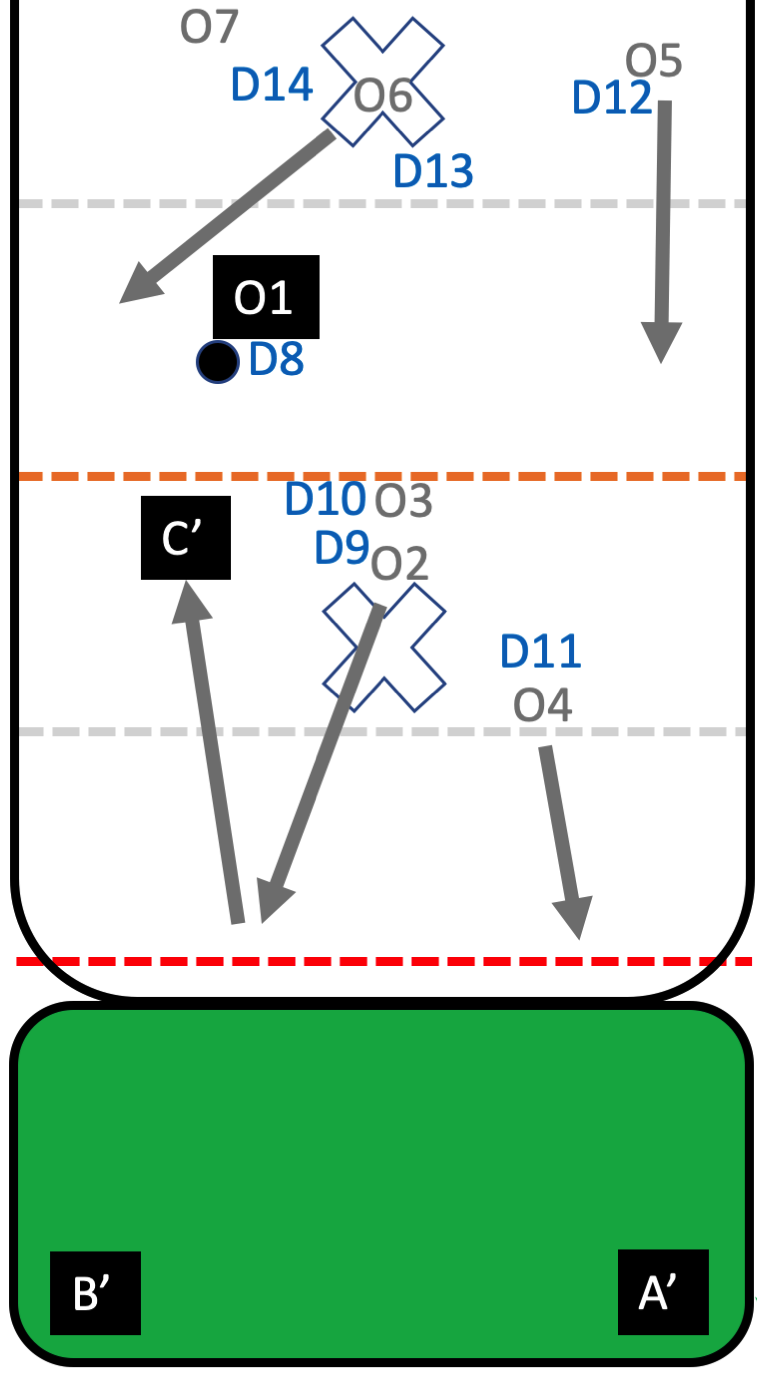
\includegraphics[width=\linewidth]{O1-vertical2}
  \caption{Vertical stack progression}
  \label{fig:O1-vertical2}
\end{marginfigure}

 In Figure \ref{fig:O1-vertical2}
your options include:
\begin{enumerate}
\item throwing to A'\footnote{
Note that A', B', C', and 
the yellow and red dashed lines 
are all now further downfield 
reflecting the new position of the disc.
The stack (O2, O3) 
has also moved downfield.}  
(to O4 or maybe O2);
\item throwing to O2 going to B' or C', 
using the same cutting approach
you did earlier;
\item off-load to O6 
moving downfield and right
as shown by the grey arrow\footnote{
A pass to O6 
should be relatively easy, 
as D13 is on the wrong side having been forcing O6 forehand earlier.   
This pass would put O6
in 'power poistion'
where they can easily 
thrown anywhere on the field 
as D13 will likely be behind them. 
In contrast, D8 
will be downfield 
of you
making it difficult to 
break the force}; 
\item break the force 
to throw to O3 
or O5; or 
\item if none of that works
throw a dump to O7
\end{enumerate}
Next, get back to the stack
or make another cut.

Other possibilities might include: 
a \smallcaps{backhand force}
(do everything the same, except the mirror image); 
a \smallcaps{straight-up force}
(it may be harder for O6 to throw to A or B, 
and it might help if 
you cut closer to the sideline 
if going upfield to C); or
\smallcaps{force middle} 
(where the force switches 
from forehand to backhand).


\begin{marginfigure}%
  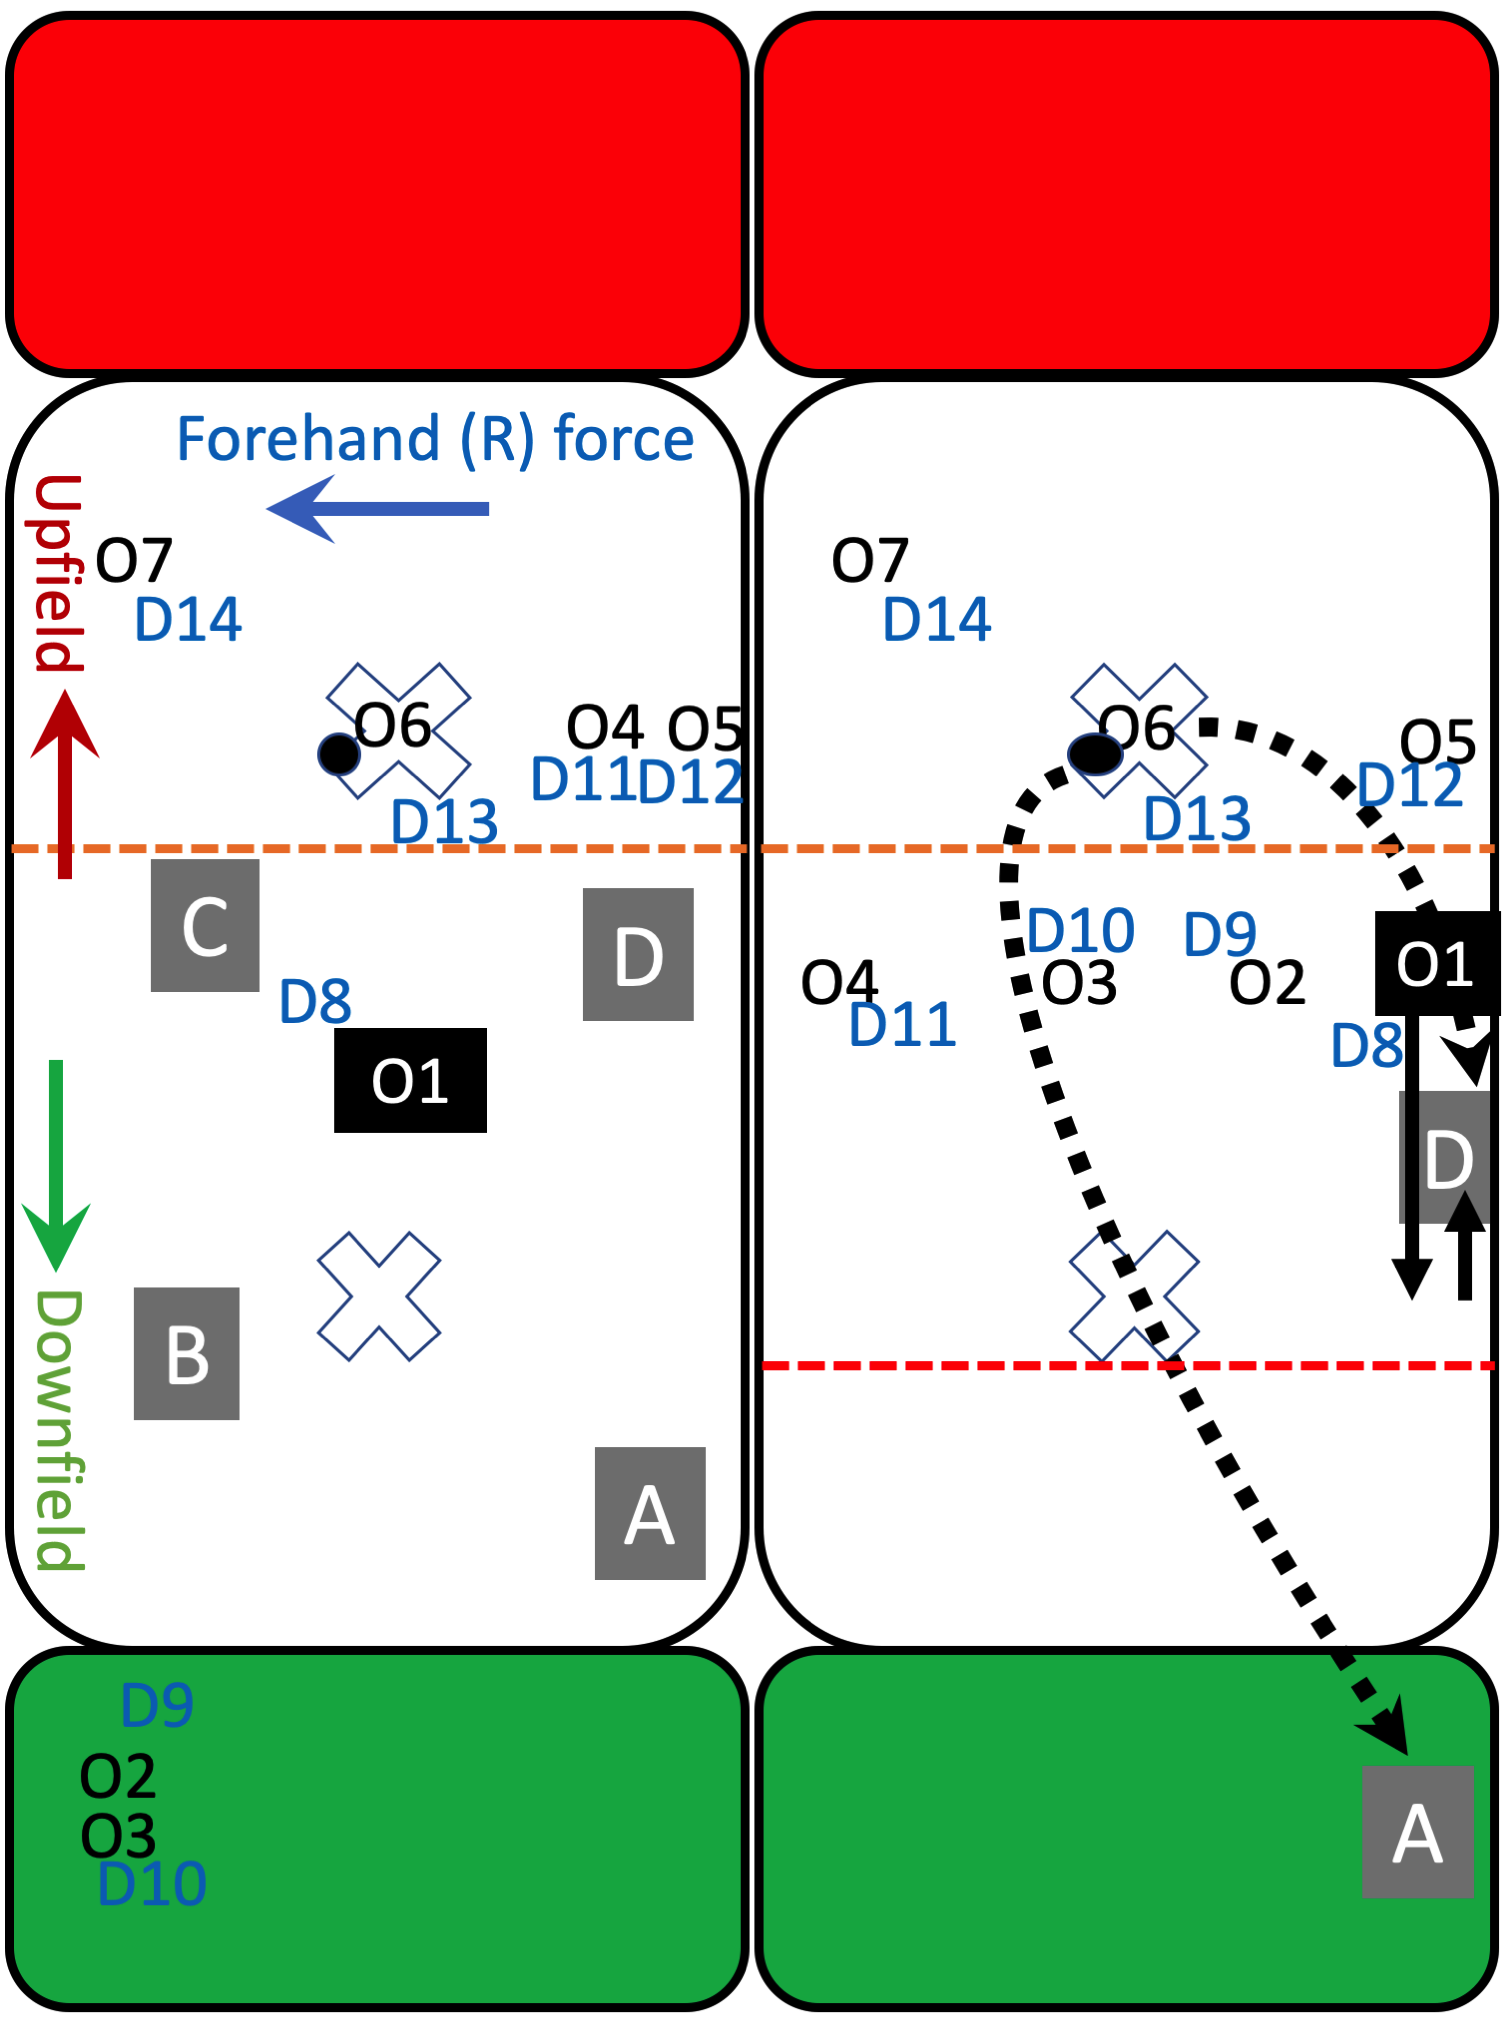
\includegraphics[width=\linewidth]{O1-horizontal}
  \caption{Horizontal stack formation}
  \label{fig:O1-horizontal}
\end{marginfigure}

\subsection{Person-match defence: horizontal stack}\label{sec:horizontall}
Figure \ref{fig:O1-horizontal} shows 
O1 on the left wing\footnote{
Typical terminology is 
as per 'stage left',
being on the left as you look downfield 
(the enemy's gate is down!)}, 
again assuming a \smallcaps{
forehand force for right handers}.
In a horizontal stack 
the strategy is to cut 
upfield and downfield (black arrows)
within your quarter of the field\footnote{
Switches to 
another quarter of the field 
can work 
(as in a diamond cut)
but usually rely on the 
other person 
(e.g. O2) 
also switching quarters 
to replace you 
on the left wing.}. 
O6 can potentially throw 
a deep huck to you downfield (A)
or a break-force throw to you (D)\footnote{
This is typically easier 
on a back-under cut, 
as shown by the black arrows,
as then there is more space 
clear of D12.}.
If you do get the disc around D, 
it is probably best 
to look to move the disc 
back to the middle of the field 
via a dump to O5 or O6, 
as it is hard to 
make progress from the sidelines 
when playing horizontal. 
In the event that 
O2, O3 or O4 
get the disc
you will be best running downfield,
to offer a deep 
or back-under cut
(probably while staying within your quarter of the field\footnote{
If O2 gets the disc,
then you
and O3 
both get a lot more space!}).


Other possibilities might include: 
a \smallcaps{backhand force}
(do everything the same, except the mirror image); 
a \smallcaps{straight-up force}
(it may be harder for O6 to throw to A or B, 
and it might help if 
you cut closer to the sideline 
if going upfield to C); or
\smallcaps{force middle} 
(where the force switches 
from forehand to backhand).




\newthought{Some key take aways} 
about vertical 
and horizontal 
stack offence 
are: 
1) you are O1, 
a cutter, 
so leave upfield of the dashed yellow lines to the handlers,
and don't go downfield of the dashed red lines 
until the disc has been thrown\footnote{
I should write extended commentaries about 
the dashed yellow 
and red lines}; 
2) standing still and letting the handler (O6) 
throw it to A\footnote{
Also, maybe the handlers might move the disc around a bit first, 
so as to get an opportunity (power position / no force) 
to take a shot towards A}
may be a reasonable option, 
especially if the handler is a good thrower, 
your defender (D8) is not 
covering you deep, or
you are faster than your defender, 
3) upfield or downfield cuts are easier to throw to
than cuts that move horizontally across the field.

\section{Zone defence}\label{sec:zone}

\begin{marginfigure}%
  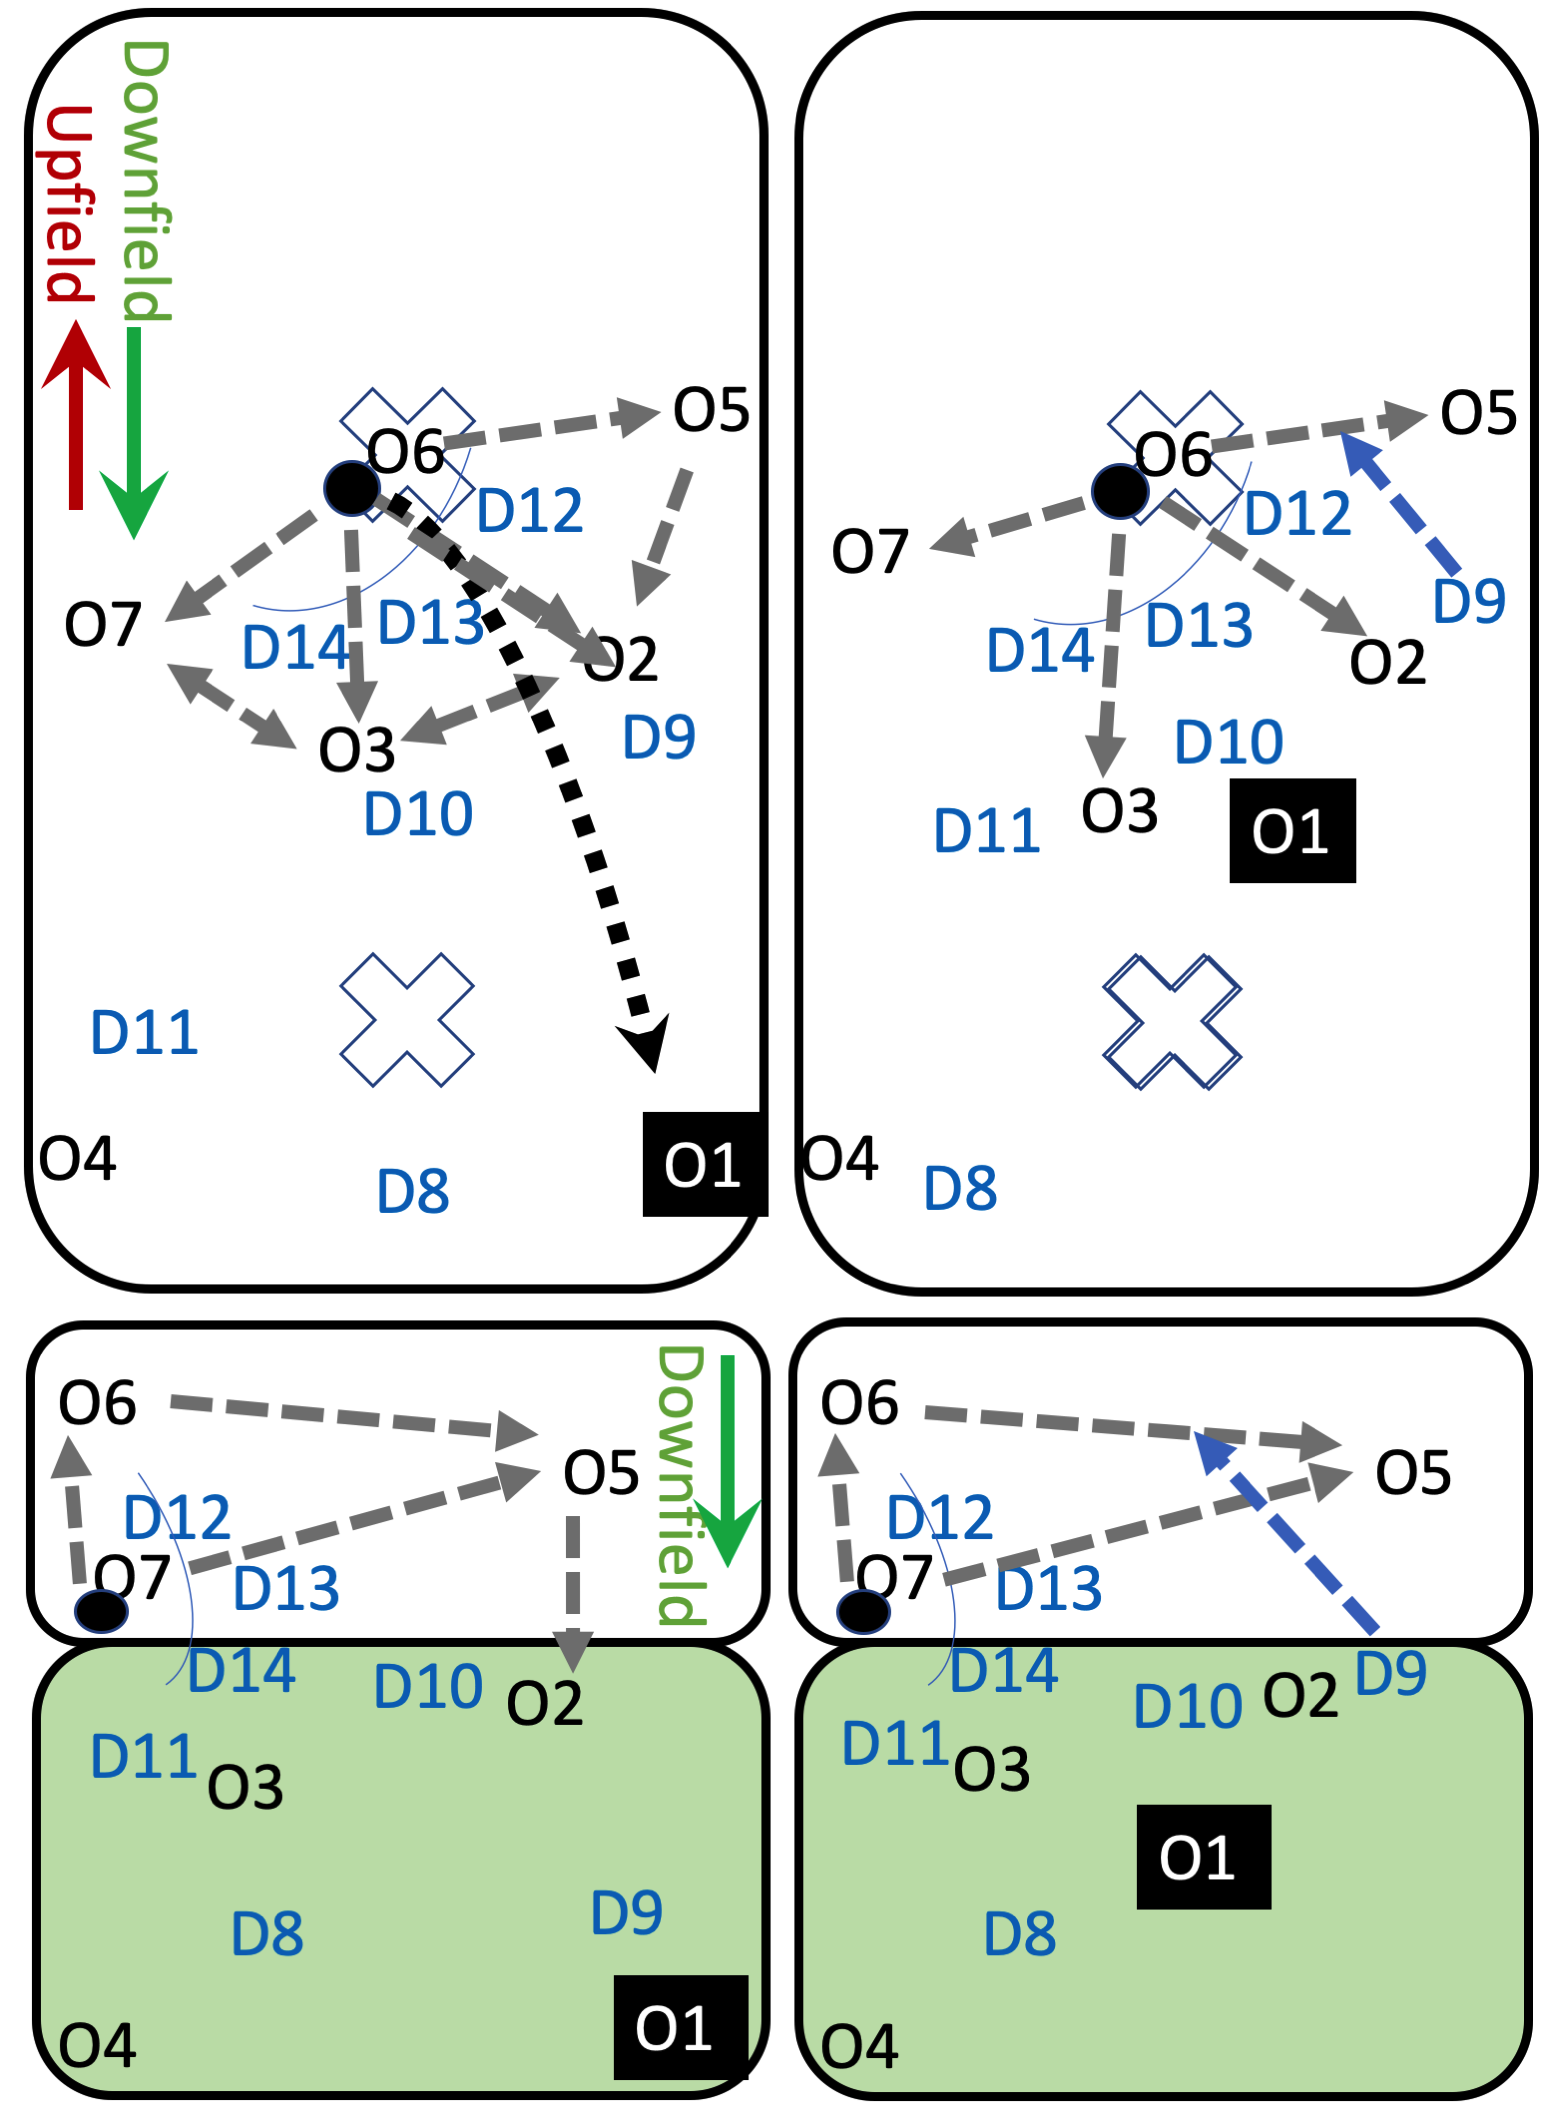
\includegraphics[width=\linewidth]{O1-zone331}
  \caption{331 zone formation}
  \label{fig:O1-zone331}
\end{marginfigure}

Oh no, 
the defence decided to play zone\footnote{
Figure \ref{fig:O1-zone331} shows a 3-3-1 zone.  
There are many other zones, 
but for the purposes of playing as O1
the principles are generally simlar.}! 
What to do? 
There are many different zones\footnote{
Even 3-3-1 might be force 
forehand, 
backhand,
middle, 
return,
sideline,
and probably more. 
Then there are 
a whole range of other formations
including:
puppy-fence (1-3-2-1),
four person cup (4-2-1)
two person cup (2,3,2) and
cup-o-saurus (6-1)!}
Regardless of what zone it is,
three ways to beat it are:
1) over;
2) round; or
3) through. 

As O1 
(left wing), 
you are mostly relevant to 
beating a zone through
(1)
\smallcaps{over}.  
This is done by exploiting the gaps between 
D8\footnote{
who is trying to cover throws 
to you or O4} 
and D9\footnote{ 
who is trying to cover you 
and O2 and 
(maybe) O5.}.
Figure \ref{fig:O1-zone331} shows 
with dashed black arrows
two potential throws from O6 to you:
\begin{enumerate}
\item O6 might throw directly to you 
(O1) where you are shown 
standing in Figure \ref{fig:O1-zone331}. 
Such a throw might be a hammer
or a blade,
because O6 will be trying to get the disc to you 
as quickly as possible, 
before either D8 or D9 can intercept it. 
Hence, it will help if you are looking directly at O6 
and standing still, 
so that they can land said throw on your head!
\item Alternatively, O6 might throw to A, 
expecting that you and the disc can get there 
before D8 does.
\end{enumerate}

The grey dashed arrows in Figure \ref{fig:O1-zone331} 
show various ways that the disc might 
go 
1) over,
2) around or
3) through 
to O5, O2 or O3. 
From them you
might receive the next pass
or the one after that
as you, collectively, 
take advantage of the 
4 (O1, O2, O3 and O5) 
versus 2 (D9 and D10)
mismatch until the 
upfield end of the zone 
(D12, D13, D14) 
catch up to the disc. 
Once they do so, 
it becomes 4 versus 5, 
so, 
as a team,
 you will likely be 
better off giving it back to 
one of the handlers 
(O5-7) 
so as to play 
7 vs 7 again. 
There are plenty of other variations,
for example, maybe it 
goes \smallcaps{(2) around}
to O7 and then deep,
taking advantage 
of the temporary 
2 (O1, O4) vs 1 (D8), 
who might have to choose 
between covering A
or B.  Regardless, 
the objective for you
as O1
is to set up 
or 2 (O1, O4) 
vs 1 (D8) 
or even 3 (O1, O4, O7) 
vs 2 (D8, D11). 
This enables your offence 
to split a defender, 
but requires that all of you
be in positions 
that can be thrown to, 
one way or another. 
Even getting a 
2 (O1, O4) 
vs 2 (D8 and D9 or D11)
downfield can be helpful, 
as then the game 
becomes 5 vs 5, 
which is easier for the offence. 


\begin{marginfigure}%
  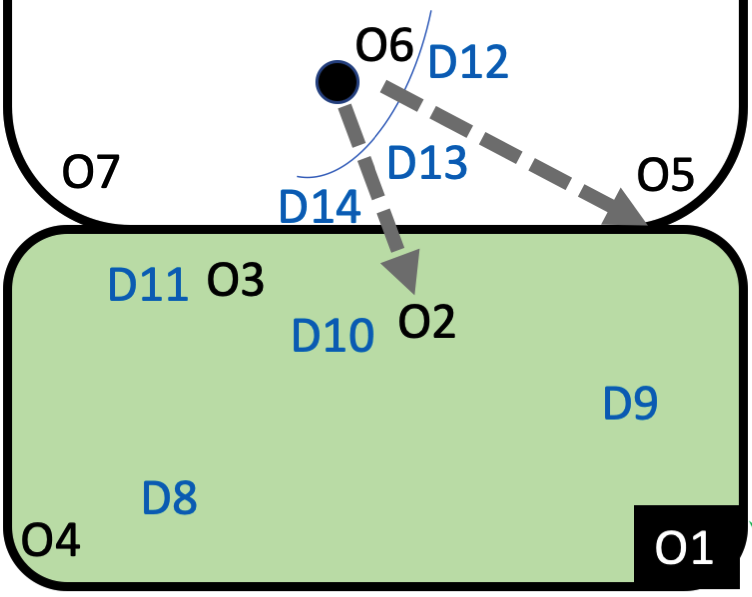
\includegraphics[width=\linewidth]{O1-zone331endzone}
  \caption{331 zone formation near the endzone}
  \label{fig:O1-zone331endzone}
\end{marginfigure}

In fact,
this should be the strategy 
if the defence 
continues to play zone 
once the disc 
gets close to the endzone, 
as shown in Figure \ref{fig:O1-zone331endzone}.
If you (O1) 
and the other wing (O4) 
go and stand 
on the back corners 
of the endzone, 
then two defenders will 
have to cover you, 
otherwise a throw \smallcaps{over}
will score\footnote{
In Figure \ref{fig:O1-zone331endzone}
D8 is shown covering O4 
(but also trying to help in the centre of the endzone)
while D9 is trying to cover O1 and O5,
and help D10 with O2.}.

\begin{marginfigure}%
  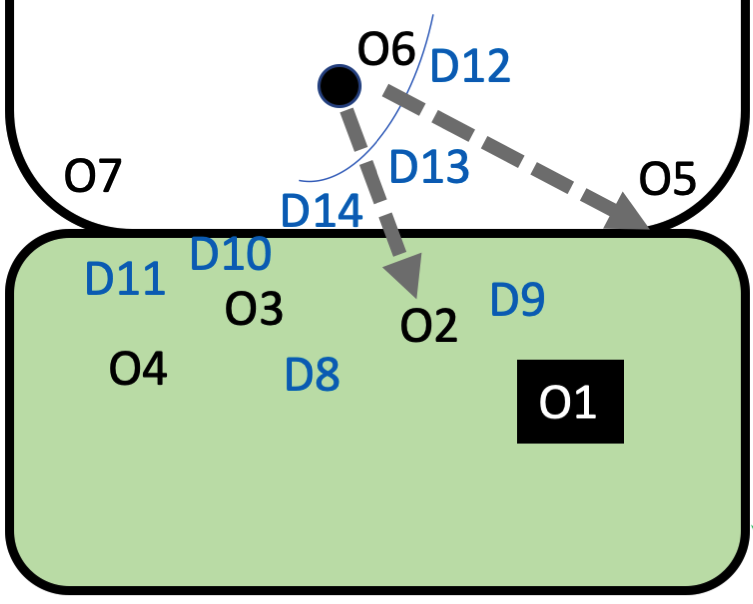
\includegraphics[width=\linewidth]{O1-zone331endzone2}
  \caption{Compressed 331 zone formation near the endzone}
  \label{fig:O1-zone331endzone2}
\end{marginfigure}

An advantage of you and O4 
being at the downfield 
corners 
of the endzone 
is illustrated through 
comparison to Figure \ref{fig:O1-zone331endzone2}.
Here O1 and O4
are further upfield
and away from the sidelines. 
This allows D8, D9, and D10 
to move upfield 
and help defend 
the front of the endzone. 
It is still possible for O6
to throw \smallcaps{over} 
into the space downfield of O1
or O4, 
however, 
this is a much harder throw. 
In Figure \ref{fig:O1-zone331endzone} 
the throw to O1 or O4 can be 
flat,
quick\footnote{
Likely, the quicker the disc gets to O1 or O4
the better,
as less time in the air 
equals less time for D8 or D9 
to get close enough to make an intercept.}
and as hard as O6 wants. 
In contrast,
the throw needed in 
Figure \ref{fig:O1-zone331endzone2} 
to pass to O1 or O4 
has to go over their (your!) head,
but be floaty enough
that it can be caught 
within the endzone. 
This appears much harder to 
throw \smallcaps{and} catch!

\section{Junk defence}\label{sec:zone}
%TALK ABOUT HOW IT'S ALL VARIATIONS ON THE THEME. FORCE THEM TO PLAY PERSON-MATCH. OR CREATE A VIABLE 2 vs 1 SITUATION.
In between zone 
and person match 
are a range of  
defensive strategies 
that are a bit of both.
The simplest is 
perhaps 
'last person back'\footnote{
In which the person who is deepest 
(furthest downfield)
switches to cover the 
offensive cutter 
who is furthest downfield 
(or the largest threat
 to receive a huck). 
The formation 
shown in Figure \ref{fig:O1-vertical} 
might involve D8 
being the 'last person back'
and so initially covering O1.  
However, once O1 
turns upfield 
D9 would switch to O1, 
with D8 subsequently covering
O2.}. 
The most complex, 
perhaps, is
'clam'\footnote{
Often called in a similar manner 
to 3-3-1 zone, 
yet with defenders effectively playing 
`person-match-with-all-the-switches'.}\footnote{
Although there's probably many 
more complex 
defensive strategies 
that I've never heard of!}.

Regardless, 
a similar approach 
to that used against zone
would seem most relevant 
to what you might do as O1. 
1) Try to spread out 
so that one defender 
cannot cover more than 
one offensive player 
(so play left wing 
and stand deep 
and wide);
2) Work with others 
on your team to try 
and find situations where 
one defender 
has to choose 
which of 2+ offensive 
players they are going to cover 
because you are arranged
such that they can't cover you all
at once!
 
That's enough for this basic document though.  
Good luck O1! 
Hopefully, 
I'll write 
more in depth 
about  zone, 
clam etc. 
in some future document. 


\end{document}
